\documentclass[a4paper]{article}
\usepackage{ctex}
\usepackage{graphicx}
\title{毕设报告}
\author{辛文钧}
\begin{document}
	\maketitle
	\begin{itemize}
		\item 实现在gazebo中用速度控制turtlebot2机器人的运动。
		\item 获得turtlebot2机器人中rostopic中的数据类型。
	\end{itemize}
	
	\section{效果图}
	\begin{figure}
		\centering
		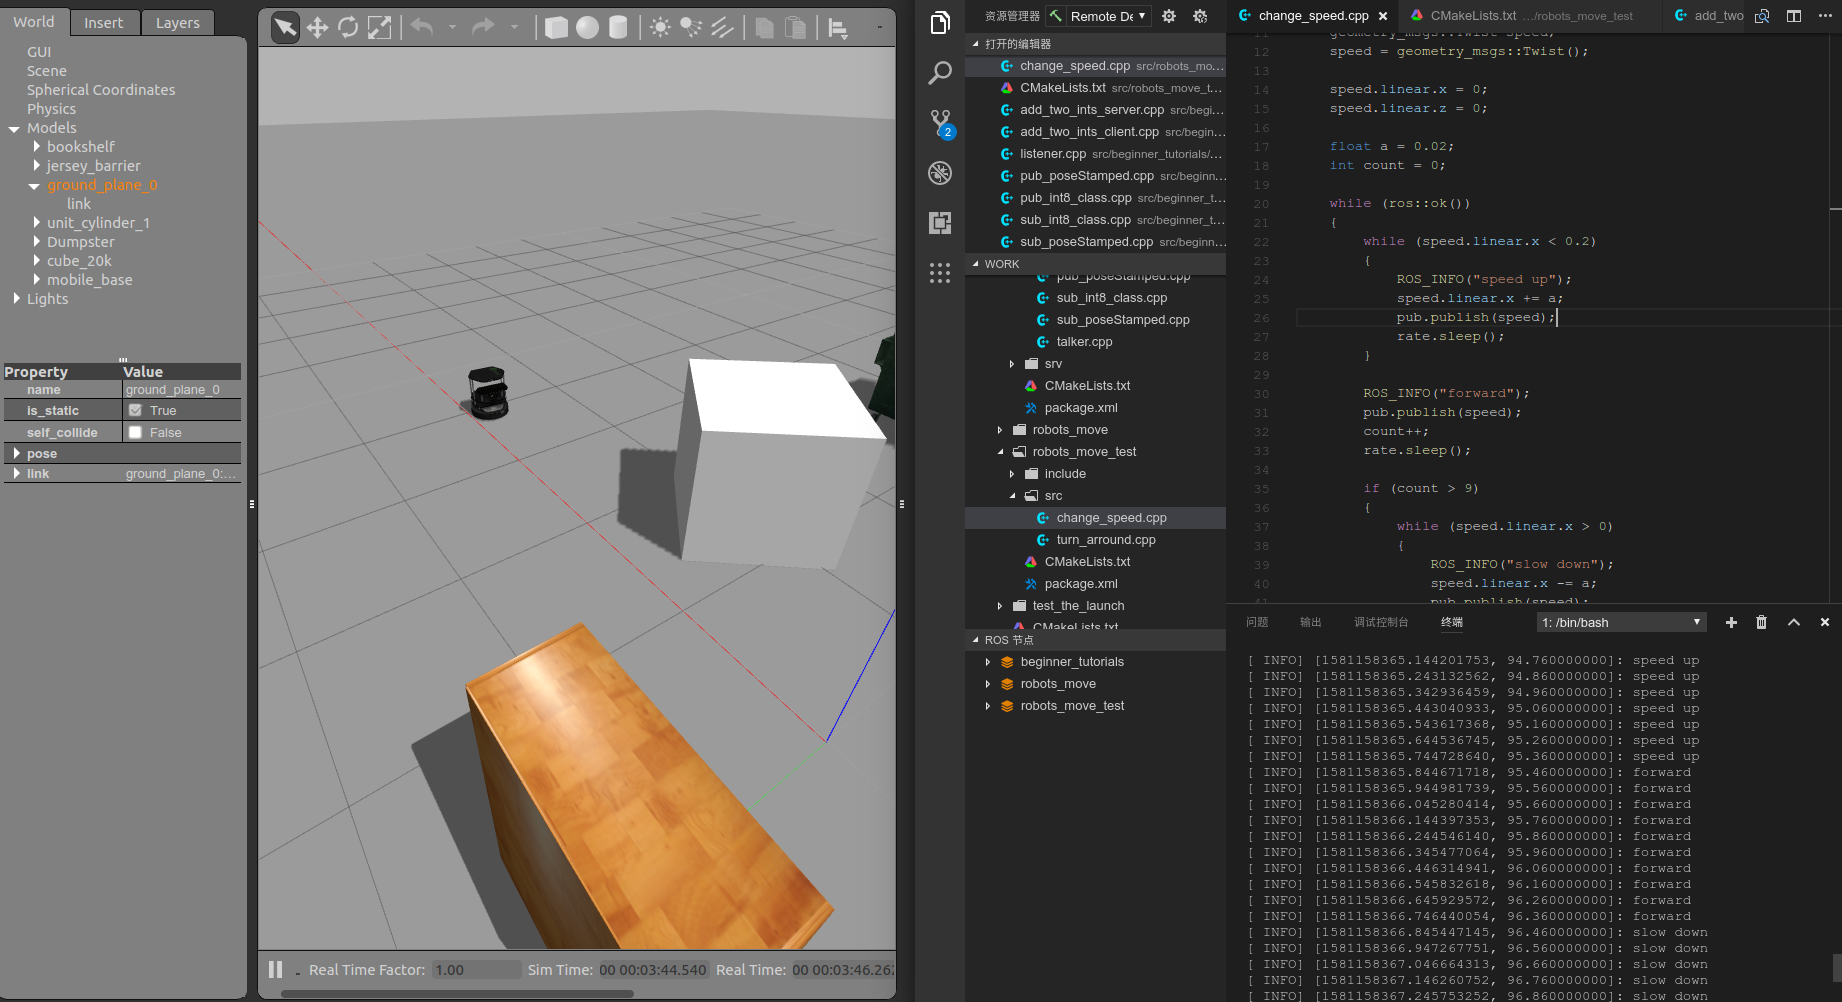
\includegraphics[scale=0.25]{move.png}
		\caption{移动效果图}
	\end{figure}
	
	\begin{figure}
		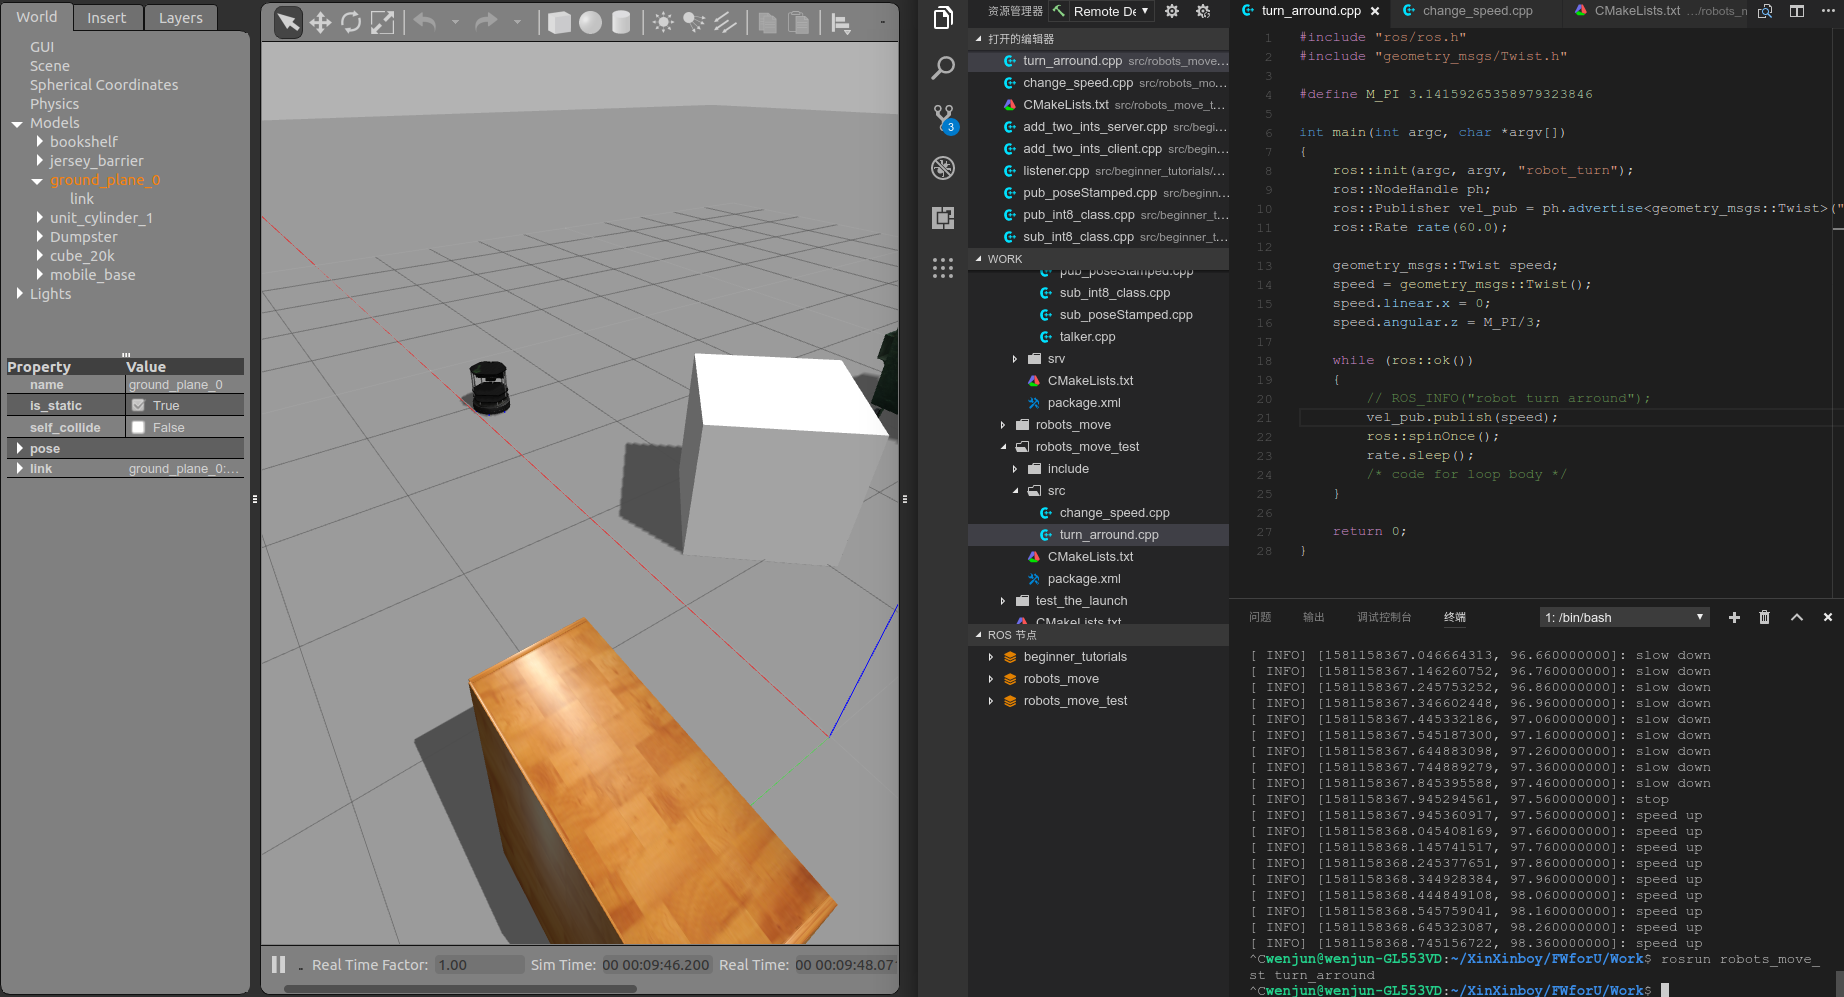
\includegraphics[scale=0.25]{turn.png}
		\caption{旋转效果图}
	\end{figure}
	
	\begin{figure}
		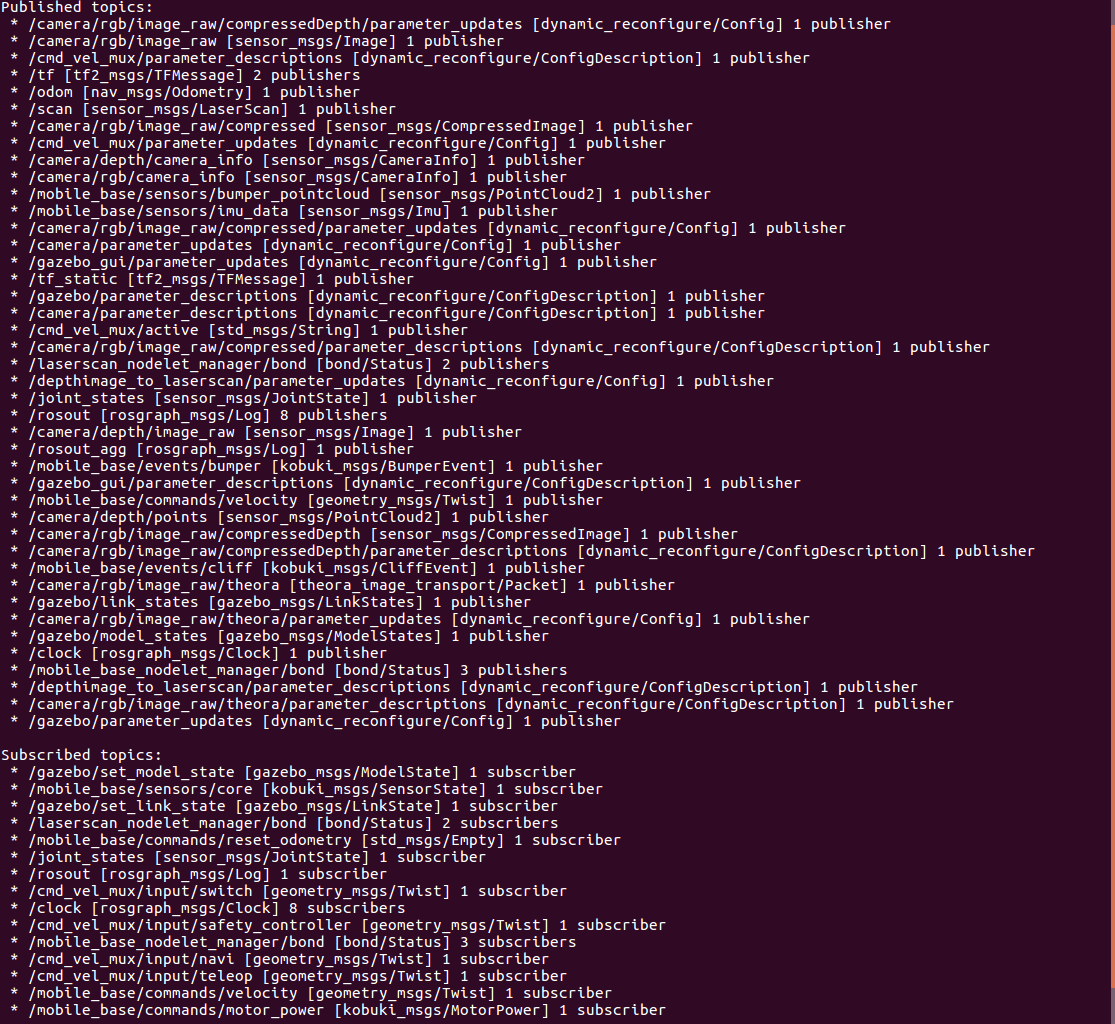
\includegraphics[scale=0.4]{turtlebot2_rostopic.png}
		\caption{turtlebot2信息}
	\end{figure}
	
\end{document}